\subsubsection{Modification de chaînes (Win32)}

Nous pouvons facilement trouver la chaîne ``hello, world'' dans l'exécutable en utilisant Hiew:

\begin{figure}[H]
\centering
\myincludegraphics{patterns/01_helloworld/hola_edit1.png}
\caption{Hiew}
\label{}
\end{figure}

Et nous pouvons essayer de traduire notre message en espagnol:

\begin{figure}[H]
\centering
\myincludegraphics{patterns/01_helloworld/hola_edit2.png}
\caption{Hiew}
\label{}
\end{figure}

Le texte en espagnol est un octet plus court que celui en anglais, nous ajoutons l'octet 0x0A à la fin
 (\TT{\textbackslash{}n}) ainsi qu'un octet à zéro.

Ça fonctionne.

Comment faire si nous voulons insérer un message plus long ?
Il y a quelques octets à zéro après le texte original en anglais.
Il est difficile de dire s’ils peuvent être écrasés: ils peuvent être utilisés quelque part dans du code \ac{CRT},
ou pas.
De toutes façons, écrasez-les seulement si vous savez vraiment ce que vous faîtes.

\subsubsection{Modification de chaînes (Linux x64)}

\myindex{\radare}
Essayons de modifier un exécutable Linux x64 en utilisant \radare{}:

\lstinputlisting[caption=\radare{} session]{patterns/01_helloworld/radare.lst}

Ce que je fais ici: je cherche la chaîne \q{hello} en utilisant la commande  \TT{/},
ensuite je déplace le \emph{curseur} (ou \emph{seek} selon la terminologie de \radare{}) à cette adresse.
Je veux être certain d'être à la bonne adresse: \TT{px} affiche les octets ici.
\TT{oo+} passe \radare{} en mode \emph{read-write}.
\TT{w} écrit une chaîne ASCII à la \emph{seek} (\emph{position}) courante.
Notez le \TT{\textbackslash{}00} à la fin--c'est l'octet à zéro.
\TT{q} quitte.

% TBT
%\subsubsection{This is a real story of software cracking}
%\label{\SoftwareCracking}
%
%An image processing software, when not registered, added watermarks,
%like ``This image was processed by evaluation version of [software name]'', across a picture.
%We tried at random: we found that string in the executable file and put spaces instead of it.
%Watermarks disappeared.
%Technically speaking, they continued to appear.
%\myindex{Qt}
%With the help of Qt functions, the watermark was still added to the resulting image.
%But adding spaces didn't alter the image itself...

\subsubsection{\emph{Traduction} de logiciel à l'ère MS-DOS}

La méthode que je viens de décrire était couramment employée pour traduire des logiciels sous MS-DOS en russe dans les
années 1980 et 1990.
Les mots et les phrases russes sont en général un peu plus longs qu'en anglais, c'est pourquoi les logiciels
\emph{traduits} sont pleins d'acronymes sibyllins et d'abréviations difficilement lisibles.

\begin{figure}[H]
\centering
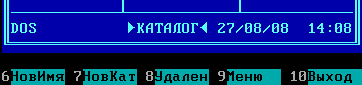
\includegraphics[width=0.5\textwidth]{patterns/01_helloworld/Norton_Commander_v5_51.png}
\caption{\FRph{}}
\end{figure}

Peut-être que cela s'est produit pour d'autres langages durant cette période.

